\chapter{Artifact Implementation}\label{chapter:artifact-implementation}

\section{Introduction}
In this chapter, I present the implementation of the primary research artifact: a collaborative augmented reality (AR) system that I designed to support co-located human-human collaboration on an industry-inspired assembly task. I designed the artifact to serve as both a functional system and a research instrument to address the second research question of this thesis: \emph{What are the challenges associated with different technical architectures for collaborative AR-based industrial task support, and how do they support multi-agent human interaction in joint task execution?}

My systematic literature review revealed a gap in understanding co-located human-human collaboration dynamics within industrial AR applications. While the field has extensively explored remote collaboration and human-robot interaction, synchronous same-space collaboration between multiple human agents remains underexplored. Existing studies focus primarily on knowledge transfer systems or precision task execution with coordination rather than collaboration.

This knowledge gap is problematic because co-located collaboration introduces unique technical and interaction challenges. Spatial misalignment between devices becomes immediately apparent to users, creating higher precision requirements for tracking systems. Real-time synchronisation latencies acceptable in remote collaboration become disruptive when users can directly observe each other's actions. Furthermore, interaction paradigms that work for single-user scenarios may interfere with natural human-human coordination patterns in shared physical spaces.

Following Hevner's three-cycle framework \cite{hevner2007dsr}, I designed the artifact to serve multiple purposes: demonstrating feasibility of co-located collaborative AR systems (design cycle), addressing practical challenges identified in the literature (relevance cycle), and contributing to theoretical understanding (rigor cycle).

I focus the implementation on identifying and implementing solutions that effectively address core collaboration requirements rather than pursuing exhaustive exploration of all possible technical architectures. This pragmatic approach prioritises functional system delivery over comprehensive architectural comparison, emphasising rapid prototyping and validation of technical components, particularly low-latency networking and shared spatial tracking.

The system was designed to support collaborative assembly tasks requiring genuine coordination between participants while maintaining measurable, quantitative outcomes. The specific task design (and the user study it supports) is detailed in Chapter~\ref{chapter:study-design}. In this chapter, I document the artifact development, analysing how technical architecture choices affect the system's ability to support multi-agent human interaction.

\section{Design Requirements}

I use the systematic literature review findings to directly inform the design requirements for the collaborative AR system. In this section, I translate key insights into specific architectural and interaction design requirements.


\subsection{Collaboration Architecture Requirements}
My analysis of collaboration types in industrial AR applications revealed four distinct archetypes, each with different architectural implications. Based on the reviewed literature, I determined that the \emph{Collaborative Creative Workflows} archetype is the most appropriate foundation for studying co-located human-human collaboration dynamics. This archetype is characterised by many-to-one synchronous information flow, where multiple users' inputs converge on shared digital objects, and direct manipulation interaction metaphors that support rapid iteration and collaborative decision-making.
I chose this archetype because it provides the richest context for studying multi-agent human interaction through genuine coordination requirements, offers a favourable balance between collaboration complexity and analytical tractability, and supports comprehensive evaluation of both task performance and collaboration quality metrics.

\subsection{User Experience Design Requirements}

My literature analysis reveals four primary UX design patterns that have proven effective in collaborative industrial AR applications. I use these patterns, combined with task-specific requirements, to inform specific design goals.

\subsubsection{Shared Spatial Context Requirements}

The literature consistently demonstrates that shared visual context is critical for successful collaboration, with studies showing superiority in both task performance and human factors metrics when users share common visual references. I therefore design the collaborative AR system to provide shared 3D spatial views where multiple users can simultaneously view and interact with the same virtual information overlaid onto their physical workspace.

This requirement extends beyond simple visual sharing to include synchronised state management, spatially aligned overlays, and real-time feedback systems that maintain visual consistency across multiple devices. I design the system to support workspace awareness mechanisms that allow users to see and understand their partners' actions and intentions, reducing miscommunication and supporting natural collaboration patterns.

\subsubsection{Direct Manipulation Interaction Requirements}

The literature reveals that while multimodal interaction interfaces can lower barriers to entry, the \emph{Collaborative Creative Workflows} archetype is most effectively supported through direct manipulation interaction metaphors that enable rapid iteration and collaborative decision-making. I therefore design the system to prioritise intuitive interaction that allows users to directly manipulate shared digital objects without requiring extensive training or cognitive overhead.

The literature also indicates that over-reliance on complex multimodal input can overwhelm users, particularly in collaborative environments where multiple interaction streams must be coordinated. I therefore implement direct manipulation as the primary interaction paradigm in the system while maintaining gesture and voice inputs as optional supplementary interaction methods.

\subsubsection{Contextual Information Display Requirements}

The literature emphasises the importance of delivering information precisely when and where it is needed, with studies showing significant improvements in situational awareness and task performance when AR systems provide contextually relevant information. I therefore design the collaborative AR system to implement spatially anchored UI elements that provide task-relevant information directly in the user's workspace, minimising cognitive load and supporting natural task flow.

I design the information display system to adapt to collaboration context, providing different information based on the current collaboration state and task requirements. This includes real-time collaboration indicators, shared attention mechanisms, and feedback systems that help users understand and coordinate their joint activities while maintaining focus on the primary creative task.

\subsubsection{Role-Based Interface Requirements}

The literature reveals that role-based interfaces and information filtering can enhance collaboration efficiency by tailoring information presentation to specific user roles and responsibilities. In collaborative industrial settings, different participants often have distinct tasks and information needs, requiring systems that can adapt interface elements and data access accordingly to avoid cognitive overload.

The literature demonstrates that role-based approaches allow for more focused and efficient collaborative workflows, with studies showing high levels of engagement and user satisfaction when interfaces provide role-specific information and system authorities. I therefore design the system to consider how different collaboration roles might require different information access, interface elements, and interaction capabilities to support effective task coordination.

\subsection{Technical Architecture Requirements}
I translate the technical challenges identified in the literature review directly into specific architectural requirements for the collaborative AR system. My analysis revealed four primary challenge categories: \emph{hardware constraints}, \emph{spatial anchoring and tracking}, \emph{network communication}, and \emph{system performance}, each requiring consideration.

\subsubsection{Hardware Platform Selection}

The overwhelming dominance of Microsoft HoloLens devices in the literature (84.4\% of studies) reflects both the maturity of the platform and the practical constraints of AR hardware availability. While HoloLens 2 offers improved ergonomics and tracking accuracy compared to the first generation, the literature consistently reports hardware limitations including restricted field of view, ergonomic constraints during extended use, and computational performance bottlenecks. These constraints directly inform the system architecture requirements. The limited field of view necessitates careful UI design, while ergonomic constraints require task structuring to accommodate realistic wearing periods. The computational limitations of the HoloLens 2 platform constrain the complexity of virtual content.

\subsubsection{Spatial Tracking and Alignment}

My literature analysis revealed that spatial anchoring and tracking represent the most persistent technical challenges in collaborative AR systems, with the majority of studies relying on headset-internal spatial anchors. However, these studies consistently reported issues with spatial drift and misalignment, particularly in dynamic environments.
I therefore implement robust spatial registration mechanisms in the artifact that address the alignment challenges identified in the literature. The evidence indicates that marker-based tracking systems provide superior accuracy and reliability for collaborative scenarios compared to headset-internal spatial anchors, despite requiring additional environmental setup. I design the system to require robust approaches for establishing shared coordinate systems across multiple headsets, ensuring that virtual content remains spatially consistent between users throughout the collaboration session.

\subsubsection{Network Communication Architecture}

Network communication challenges emerge as critical factors affecting collaboration quality, with the literature revealing that even sophisticated custom networking solutions may encounter significant issues when scaling to multiple concurrent users. My analysis indicates that communication latency is more critical than bandwidth requirements. I therefore implement a networking architecture in the artifact that is optimised for low-latency state synchronisation rather than focussing on high bandwidth.

\section{Core Technical Architecture}
Based on the requirements outlined above, I implemented the artifact as a modular \textbf{MRTK3}\,/Unity~6 application targeting Microsoft HoloLens 2.  
Core functionality is mostly encapsulated in a singleton \texttt{MonoBehaviour} —\texttt{ObjectManager}. As a single managing entity, it includes the foundational networking, spatial tracking, and object synchronisation components. This pattern provides loose coupling (individual components can be replaced without affecting the overall system, even though they are attached to the same GameObject) while avoiding the complexity of a full \texttt{ScriptableObject} service-locator architecture.

\subsection{Networking}\label{subsec:networking}

\begingroup
  \setlength{\tabcolsep}{4pt}
  \renewcommand{\arraystretch}{1.05}

\begin{sidewaystable}[htbp]
  \centering
  \scriptsize
  \caption{Unity networking middleware compared for co-located Augmented Reality (AR) applications (2025 audit)}
  \begin{tabular}{@{}
    >{\raggedright\arraybackslash}p{2.1cm}
    >{\raggedright\arraybackslash}p{2.3cm}
    >{\centering\arraybackslash}p{0.8cm}
    >{\raggedright\arraybackslash}p{1.6cm}
    >{\raggedright\arraybackslash}p{1.9cm}
    >{\raggedright\arraybackslash}p{2.1cm}
    >{\raggedright\arraybackslash}p{1.9cm}
    >{\raggedright\arraybackslash}p{2.5cm}
  @{}}
  \toprule
  \textbf{Solution} & \textbf{License / Cost} & \textbf{Open Src} &
  \textbf{Authority Model} & \textbf{Local LAN / P2P} &
  \textbf{Platform Scale\textsuperscript{\dag}} & \textbf{Latency compensation} &
  \textbf{Notable Traits} \\
  \midrule
  Netcode for GameObjects\footnote{\url{https://unity.com/products/netcode}} &
    Unity Companion; UGS pay-as-you-go & yes (Unity Companion License) &
    client-server &
    Relay (official) or experimental LAN sample &
    No built-in cap\footnote{\url{https://docs-multiplayer.unity3d.com/netcode/current/basics/max-players/}} &
    snapshot + prediction &
    Official Unity stack \\[2pt]

  Mirror\footnote{\url{https://mirror-networking.com/}} &
    MIT; free & yes &
    client–server / host-client &
    Built-in \texttt{NetworkDiscovery} &
    No built-in cap\footnote{\url{https://github.com/MirrorNetworking/Mirror}} &
    tick-buffer; manual comp &
    Huge OSS user base \\[2pt]

  Photon PUN 2\footnote{\url{https://www.photonengine.com/pun}} &
    SaaS; free 20 CCU then tiered & no &
    client-server (Photon Cloud) &
    \emph{Deprecated} Photon LAN - via cloud relay &
    Default 16; higher only by request\footnote{\url{https://doc.photonengine.com/pun/current/troubleshooting/faq}} &
    adaptive tick &
    Mature docs; voice \& analytics bundle \\[2pt]

  Photon Fusion\footnote{\url{https://www.photonengine.com/fusion}} &
    SaaS; free 100 CCU & no &
    host-sync or server &
    LAN + colocation sample &
    Configurable; default 16\footnote{\url{https://doc.photonengine.com/fusion/current/manual/playerref}} &
    rollback + prediction &
    Tuned for XR at 60-120 Hz \\[2pt]

  Normcore\footnote{\url{https://normcore.io/}} &
    Free Public tier (100 room-hours + 120 GB/mo)  & no &
    server-authoritative &
    on-prem (paid) &
    4-250 per room\footnote{\url{https://docs.normcore.io/room/room-server-options}} &
    20 Hz default (configurable → 90 Hz) &
    Voice + avatars out of the box \\[2pt]

  Fish-Networking\footnote{\url{https://fish-networking.gitbook.io/docs}} &
    MIT; free & yes &
    server or P2P (via 3rd-party transports) &
    LAN discovery helpers &
    No built-in cap\footnote{\url{https://fish-networking.gitbook.io/docs/manual/general/performance/fish-networking-vs-mirror}} &
    built-in lag comp &
    High-perf; active OSS since 2022 \\[2pt]

  DarkRift 2\footnote{\url{https://github.com/DarkRiftNetworking/DarkRift}} &
    Mixed (MPL-2.0/MIT); free (paid support) & yes &
    server-authoritative &
    custom impl &
    No built-in cap\footnote{\url{https://github.com/DarkRiftNetworking/DarkRift}} &
    deterministic message pump &
    Ultra-low GC; headless C\# server \\
  \bottomrule
  \end{tabular}
  \label{tab:net_survey_ar}

  \vspace{1ex}
  \footnotesize\textsuperscript{\dag}"Platform Scale" figures are theoretical maximums from vendor documentation; actual achievable CCU depends on game design, hardware specifications, and network conditions.
\end{sidewaystable}

\endgroup

\paragraph{Middleware selection}
Table~\ref{tab:net_survey_ar} surveys seven Unity networking stacks against co-located AR requirements.  While initially PUN2 was considered, it was later replaced with Fish-Net (open-source) combined with the Tugboat local networking stack, due to its inability to cope sufficiently with a suboptimal network connection.

\paragraph{Physical network setup}
For the user study deployment, I set up a dedicated WiFi router supporting 5GHz band (TP-Link Archer MR200) to ensure reliable network connectivity. I connected all devices to this controlled network environment. I configured the system to run three instances of the software concurrently: two on the HoloLens 2 headsets worn by participants, and one on a laptop that served as the network host, providing centralised control of the environment and participant observation capabilities.

\paragraph{Authority model}
In collaborative experiences, where users are interacting with the same physical objects, determining which network node controls shared objects is critical for maintaining consistency and preventing conflicts. I implement a hybrid authority model in the artifact where a dedicated laptop host runs the authoritative physics simulation while HMDs act as semi-authoritative clients. Ownership is transferred implicitly once a user interacts with an object:

\begin{enumerate}
  \item grab $\rightarrow$ client gains ownership,
  \item transient cascade $\rightarrow$ touching rigidbodies inherit ownership for a few physics frames,
  \item release $\rightarrow$ host regains ownership.
\end{enumerate}

The scheme maintains deterministic collision resolution while enabling latency-free local prediction on the grabbing client.

\paragraph{Network throughput}
The client tick rate is 120 Hz, with a server-side tick rate of 500 Hz. Maximum MTU in Fishnet was set to 1024 bytes, though actual payload size may be lower.
In local benchmarks, the average inbound (server-to-client) bandwidth is 0.16 $\pm$ 0.31 kbps while outbound (client-to-server) bandwidth is 1.26 $\pm$ 2.51 kbps for two users, with 99th percentile values of 0.80 kbps and 6.32 kbps respectively. This represents minimal sustained throughput requirements, providing substantial headroom for eight HMDs on a commodity access point. Average round-trip latency is 25.72 $\pm$ 8.85 ms on localhost with 99th percentile at 85.00 ms. Assuming additional wireless networking latency of 10 ms on a 5GHz Wi-Fi 6 access point (\cite{liu2023wifi} claims under 6 ms on a mostly clean spectrum), the total latency is 35.72 $\pm$ 8.85 ms—well within the commonly accepted 50 ms latency target for real-time interactive systems \cite{sonkoly2024edge}.

Latency spikes are further masked by FishNet's \emph{adaptive interpolation buffer}, which automatically widens from two to three ticks when the measured half-round-trip time increases, absorbing transient jitter without visible artefacts. Immediate local responsiveness is maintained by client-side prediction combined with authoritative state reconciliation (a client simulates its own input every tick, while the server echoes the authoritative result; any divergence triggers a lightweight rollback and re-simulation that completes inside the same video frame). Finally, all transform snapshots are delta-compressed against the last acknowledged baseline and batched into a single UDP packet per tick, so the typical packet payload remains only a few dozen bytes, easily fitting within the theoretical maximum 1024-byte MTU \cite{fishnetDocs2024, dobson2024lagcomp}.

\begin{figure}[t!]
  \centering
  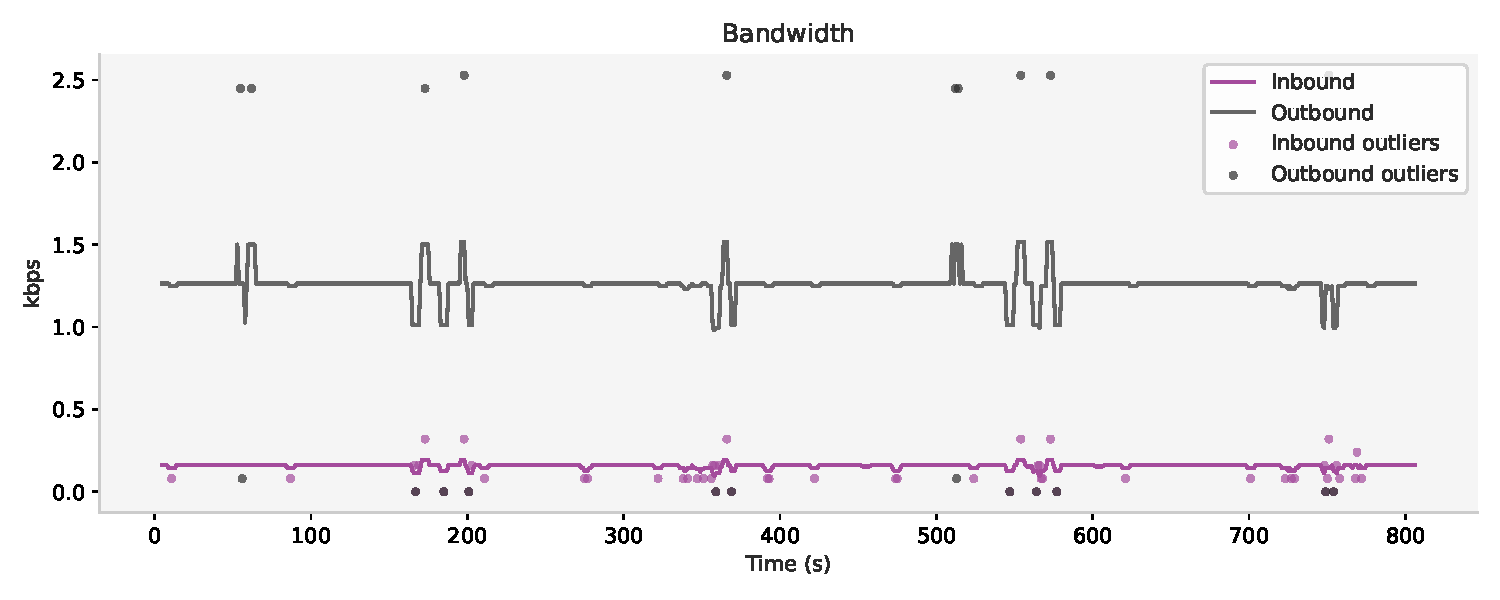
\includegraphics[width=0.8\textwidth]{assets/04/bandwidth.pdf}
  \caption{Network bandwidth utilisation over time (on localhost).}
  \label{fig:bandwidth}
\end{figure}

\begin{figure}[t!]
  \centering
  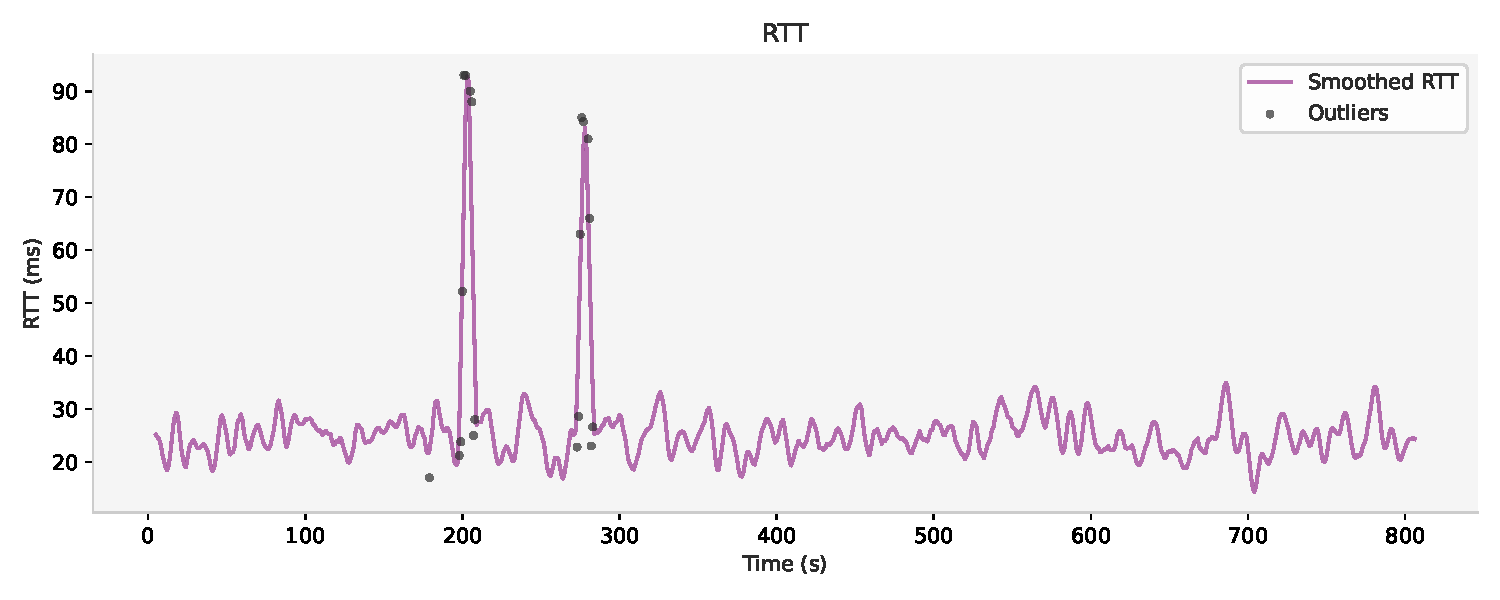
\includegraphics[width=0.8\textwidth]{assets/04/rtt.pdf}
  \caption{Round-trip time (RTT) measurements (on localhost).}
  \label{fig:rtt}
\end{figure}


\subsection{Shared-space Spatial Anchoring}\label{subsec:anchoring}
In a co-located setting, localisation becomes both harder and more important. Harder because aligning multiple devices at the required precision is harder, and room for error is smaller (as misalignments are more visible when users expect to be able to seamlessly points at, pick up and place objects in the same shared space environment). More importantly, while in a single-user or remote setting, minor misalignments or drifts rarely impact the usability of the system, they quickly ruin the experience in a co-located setting.

To that end, I experimented with various different localisation approaches. In general, the process of localisation can be broken down into two main steps:
\begin{enumerate}
    \item \textbf{Setting and recognizing anchors}: recognizing the markers on the floor.
    \item \textbf{Positioning the devices}: using the virtual anchors to position the devices in the shared space.
\end{enumerate}

For the former, I initially experimented with Azure Spatial Anchors, but due to its retirement in late 2024\footnote{\url{https://learn.microsoft.com/en-us/lifecycle/products/azure-spatial-anchors}}, was forced to switch to more traditional marker-based tracking.
Marker-based tracking, by contrast, continues to deliver sub-millimetre precision in assembly scenarios, provided that lighting is controlled. As a result, I performed all evaluations carried out during the user study in a controlled environment lit by overhead LED panel lights.

\paragraph{Anchor rig and detection}
Three Vuforia image targets (A4 laser prints on matte paper, 24 x 18 cm each; see appendix \ref{appendix:anchors}) were positioned on the play space floor. 
In earlier testing, I benchmarked ArUco 4x4 tags, Vuforia image targets, and VuMarks with the Vuforia SDK; out of these, Vuforia yielded noticeably steadier pose estimates on both the simulator (using a webcam) and HoloLens 2.

\paragraph{Two-stage calibration (“lock-in”)}
Because Vuforia is a black-box SDK, there is little that can be done to further improve tracking performance for each timepoint. Therefore, I design the system to perform a short, robust calibration that (i) aggregates noisy Vuforia poses into three high-confidence marker poses and (ii) fixes a stable, device-independent playspace coordinate frame whose origin is the centroid of the marker constellation.

\begin{enumerate}
    \item \textbf{Raw sampling.}\;
          For each planar fiducial marker (image target) $\mathcal M_k \;(k=1,2,3)$ the Vuforia SDK
          streams $N = 30\,\text{Hz}\times 5\,\text{s} = 150$ pose estimates
          \(\{(\mathbf p_{ki},\mathbf R_{ki})\}_{i=1}^{N}\), where
          \(\mathbf p_{ki} \in \mathbb R^{3}\) and
          \(\mathbf R_{ki}\in SO(3)\).
    
          \item \textbf{Per-marker “lock-in’’.}\;
          From the $N=150$ noisy pose samples of a single marker
          \(\{(\mathbf p_{ki},\mathbf R_{ki})\}_{i=1}^{N}\) a single,
          high-confidence pose is extracted:
    
          \[
            \mathbf p_k = \operatorname{gmedian}\bigl\{\mathbf p_{ki}\bigr\},
            \qquad
            \mathbf R_k = \operatorname{mean}_{SO(3)}\bigl\{\mathbf R_{ki}\bigr\}.
          \]
          \textbf{Geometric median.}  
          Considering the position samples as a set of points in $\mathbb R^{3}$,
          the geometric median is the point that minimises the total
          straight-line distance to every point in the set,
          \(\sum_i\|\mathbf p-\mathbf p_{ki}\|\).
          Compared with the ordinary (arithmetic) mean it is far less sensitive
          to outlier values. More than half of the samples must be
          corrupted before the estimate can be pulled arbitrarily far away
          (\(>50\%\) breakdown point).
    
        \textbf{Intrinsic (Karcher) mean on \(SO(3)\).}  
          Rotations form the curved three-dimensional manifold
          \[
            SO(3)=\{\mathbf R\!\in\!\mathbb R^{3\times3}\mid
                   \mathbf R^{\!\top}\mathbf R=\mathbf I,\;
                   \det\mathbf R=1\}.
          \]
          A naive, element-wise average of the nine matrix entries would leave
          this surface and yield something that is no longer a valid rotation.
          The Karcher mean avoids that by averaging along the manifold:
          each sample is first projected into a local tangent plane, averaged
          there, and the result is then mapped back onto \(SO(3)\).
          This shortest-path (geodesic) averaging keeps
          \(\mathbf R_k\) inside \(SO(3)\) while still damping out noise and
          outliers.
    
          Together, the geometric median for translation and the Karcher mean
          for rotation provide a robust approximation of each
          marker's true pose.
    
        
    \item \textbf{Virtual origin.}\;
          The playspace origin is anchored at the centroid of the locked-in
          marker centres:
          \[
            \bar{\mathbf p}\;=\;\tfrac13(\mathbf p_1+\mathbf p_2+\mathbf p_3),
            \qquad
            \mathbf t\;=\;-\bar{\mathbf p}.
          \]
          This choice removes any dependence on external world coordinates and
          guarantees that the headset is centred within the marker triangle.
    
    \item \textbf{Canonical orientation.}\;
    Marker $\mathcal M_1$ acts as a fixed \emph{forward} reference.
    Let \(\mathbf p_1\) and \(\mathbf R_1\) be its locked-in
    centre and rotation; the marker normal is
    \(\mathbf n_1\) (e.g.\ the third column of \(\mathbf R_1\)).
    With the origin at \(\bar{\mathbf p}\) an orthonormal, right-handed
    basis is obtained by
    \[
      \hat{\mathbf z}=\mathbf n_1,\qquad
      \hat{\mathbf x}=\frac{\mathbf p_1-\bar{\mathbf p}}
                           {\|\mathbf p_1-\bar{\mathbf p}\|},\qquad
      \hat{\mathbf y}=\hat{\mathbf z}\times\hat{\mathbf x},
    \]
    \[
      \mathbf R=[\,\hat{\mathbf x}\;\hat{\mathbf y}\;\hat{\mathbf z}\,].
    \]
    This locks the $x$-axis to the ray from the centroid to
    \(\mathcal M_1\) and the $z$-axis to the physical normal of
    \(\mathcal M_1\), yielding a reproducible orientation across
    sessions.    
    
    \item \textbf{Headset-playspace alignment.}\;
    After lock-in the virtual-camera (inside Unity) is shifted to the inverse
    calibration pose  

    \[
      T_{\text{rig}}
      \;=\;
      \begin{bmatrix}
        \mathbf R^{\!\top} & -\mathbf R^{\!\top}\bar{\mathbf p}\\[2pt]
        \mathbf 0^{\!\top} & 1
      \end{bmatrix},
    \]

    where  

    \begin{itemize}
    \item \(\mathbf R\) is the canonical playspace basis expressed in
      headset coordinates, and  
    \item \(\bar{\mathbf p}\) is the centroid of the three locked-in marker
      centres.
    \end{itemize}

    The rig is therefore (i) translated so the centroid lands at the playspace origin and (ii) counter-rotated so the headset's axes are brought into exact agreement with the playspace axes.
  
    \end{enumerate}

\paragraph{In-session verification}
After the playspace has been established, the two players are asked to perform a brief mutual check by standing at the edge of the playspace and looking at each other's head:
    \begin{enumerate}
    \item \textbf{Visual target.}\;
          Each wearer sees a $\varnothing5\,\mathrm{cm}$ white disk centred on the partner's face, idealised below as a circular region of radius $R=7\,\mathrm{cm}$ (this equals a head diameter of 14 cm).
    
    \item \textbf{Pass criterion.}\;
          Alignment succeeds when the marker lies entirely inside the facial disk (“Is the white dot on the other player's head?”). Geometrically, this limits the total (combined) in-plane offset of the two centres to
          \[
            s_{\max}=R-r\;=\;70\,\mathrm{mm}-25\,\mathrm{mm}=45\,\mathrm{mm}.
            \tag{1}\label{eq:smax}
          \]
    
    \item \textbf{Guaranteed accuracy at $d=2.5\,\mathrm m$.}
          If the test is passed, the residual mis-registration is bounded by
          \[
            \boxed{\|\Delta\mathbf t_{\perp}\|\;\le\;45~\text{mm}},
            \qquad
            \boxed{\|\Delta\mathbf R\|_{\angle}\;\le\;
                   \frac{s_{\max}}{d}= \frac{45\,\mathrm{mm}}{2.5\,\mathrm{m}}
                   \approx 0.018\;\text{rad}\;(1.03^{\circ}) }.
            \tag{2}\label{eq:bounds}
          \]
    \end{enumerate}
    
    These $\le\!4.5\text{ cm}$ translation and $\le\!1.03^{\circ}$ rotation limits are theoretical worst-case guarantees. The additional benefit of this test is that it allows understanding \emph{how} the system is misaligned, which is useful for debugging and improving the system.

\paragraph{Runtime behaviour and drift}
No significant drift was observed over the course of the play sessions, which lasted a maximum of around 30 minutes. In two instances participants noted minor discrepancies in alignment, but these were not significant enough to impact the task. On the other hand, moving the headsets out of the designated play space (e.g.\ to the charging station) degraded internal SLAM enough that a recalibration was usually required.
Shorter lock-in countdowns and on-the-fly re-calibration on marker-detection were tested but produced either higher jitter or intrusive visual disruptions, so the full pre-round procedure was retained.

\subsection{Spatial UI Design}
Designing interface elements that two HoloLens 2 users can read, reach, and ignore when appropriate is a non-trivial task. Early versions of the artifact employed palm-anchored tool palettes inspired by on-hand menus shown to be efficient in single-user AR scenarios \cite{azai2018openPalm}. In practice, however, the menus were often either triggered accidentally (pure gesture-based activation) or were hard to trigger (when requiring eye-gaze activation) and designing for ambidextrous users proved challenging.

\begin{figure}[h]
    \centering
    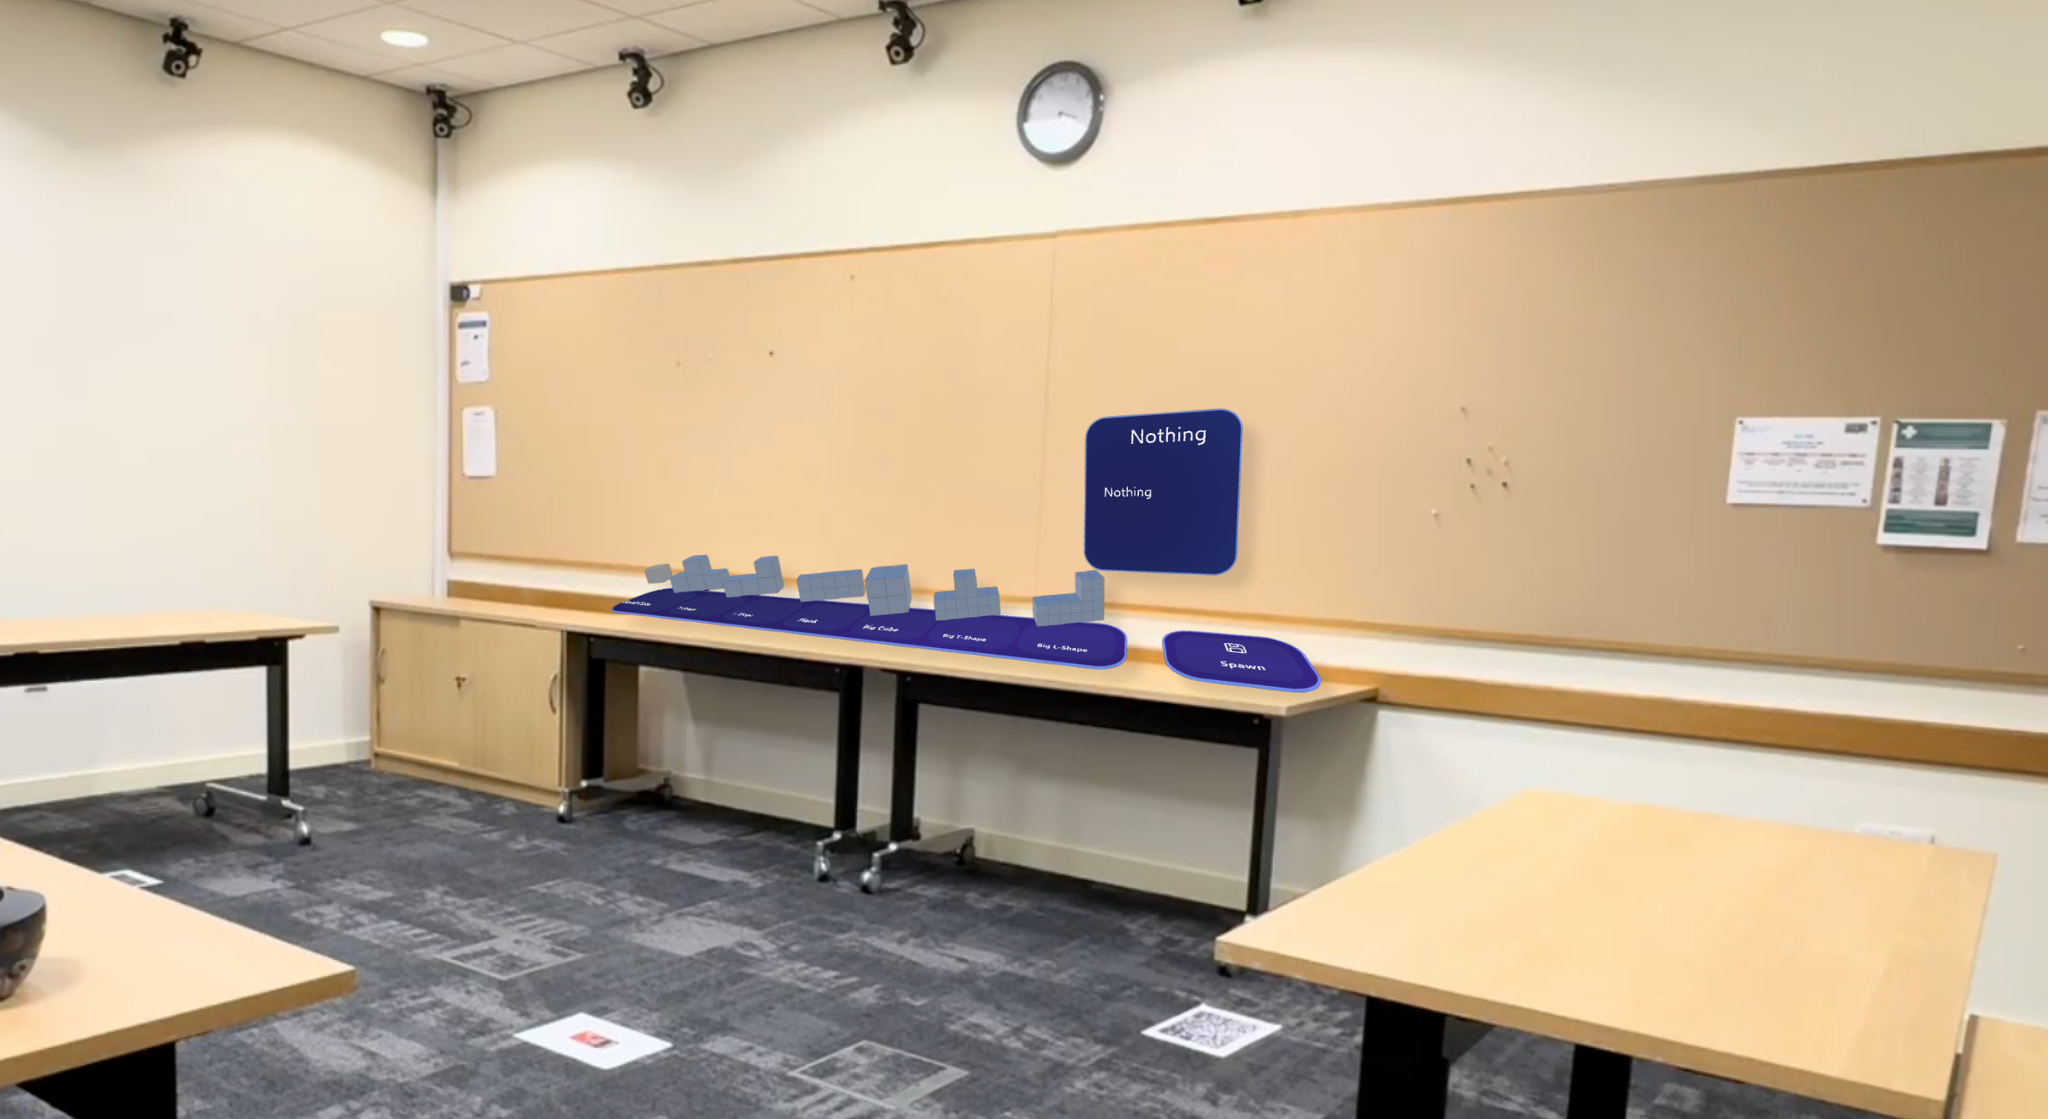
\includegraphics[width=0.8\textwidth]{assets/04/menu-in-room.png}
    \caption{Virtual UI positioned on physical table (conceptual illustration with real UI asset)}
    \label{fig:menu-in-room}
\end{figure}

Guided by \cite{billinghurst2005designing}'s observation that world-anchored virtual controls lower the cognitive overhead of AR interaction, I relocated all interactive controls to virtual boards positioned on top of real tables (see figure \ref{fig:menu-in-room}). The boards are positioned at opposite ends of the workspace so users can reach their own controls without interfering with their partner.

Each interactive "spawn" button includes a brief countdown timer that disables further activation until the current spawn operation completes, preventing accidental multiple spawns when users rapidly pressed buttons. This simple mechanism eliminated the common issue of users accidentally creating multiple identical parts when they pressed buttons in quick succession, improving both system stability and user experience.

Deletion zones followed a similar iterative path. A first-pass solution, instantly removing a part when it enters a red-zone attached to the hand-tracking menu, again caused accidental deletions and confusion. The final design introduces a set of red, semi-transparent zones rendered on the floor, that simultaneously serve to vary the task (by introducing zones where no blocks may be placed). A part placed in the red zone is removed after a 3 second grace period, and emits a spatialised audio cue before disappearing.

\subsubsection{Limitations}
While the spatial anchoring system demonstrates robust performance within its design parameters, it requires each HMD to independently complete its own calibration procedure against the physical marker constellation as anchors are not shared between devices. This approach ensures that each device establishes its own high-confidence spatial reference frame through the two-stage calibration process, though it does require coordinated setup procedures for multi-user sessions.

During extended play sessions lasting up to 30 minutes, the system maintained stable spatial registration without requiring intervention. However, moving headsets outside the designated play area for charging or storage between sessions typically degraded the internal SLAM tracking sufficiently to warrant recalibration. This behaviour led to the adoption of a consistent pre-session calibration protocol that, while ensuring optimal spatial alignment at the start of each task variant, introduced an additional step into the study protocol and lengthened the total session duration.

\subsection{Building System}
The user study described in Chapter \ref{chapter:study-design} requires participants to collaboratively construct bridge-like structures from virtual blocks. A collaborative building system is required to support that task. This section summarises the key design decisions and UX lessons learned during the development of this building interface.

The first prototype, inspired by MRKT3 example scenes\footnote{\url{https://learn.microsoft.com/en-us/windows/mixed-reality/mrtk-unity/mrtk3-overview/getting-started/exploring-features/mrtk3-sample-scenes}}, allowed free-form placement of blocks via direct manipulation. In practice, it was nearly impossible to build a stable span. Slight misalignments combined with gravity and Unity's default collision resolution caused frequent collapses, leading to frustration and repeated rebuilds, even in single-user scenarios.

\paragraph{Placement stability.}
The primary fix to mitigate alignment errors was to introduce an explicit placement grid: whenever a block was released, its position snapped to the nearest 5 cm grid cell, accompanied by a brief alignment animation to reinforce the anchoring. This improved alignment precision but did not succeed to eliminate collapses fully. Consequently, the physics model was augmented with a two-stage weighting scheme:
\begin{itemize}
\item In-motion damping: while a block is being moved, its effective mass is reduced to 10 \% of its final value, making it easier to slide into place without imparting large impulses to neighbouring blocks.
\item Static reinforcement: once stationary and supporting another block, its effective mass increases to 10 times its nominal weight, greatly enhancing the stability of lower layers.
\end{itemize}
The combination of animated grid snapping and dynamic mass adjustment in the final artifact effectively reduced accidental knock-overs, and allowed for the construction of persistent structures that survived normal collaborative manipulation.

\paragraph{Pickup feedback}
A common HoloLens gesture pattern allows users to "air-tap" at a distance to grab objects. In early tests, one user's distant pick-up actions were invisible to their partner, causing confusion when objects started moving without being picked up from the other's view. To address this, any block currently held by either user is highlighted with a glowing blue tint.

\section{Bridge Evaluation Methodology}

To provide objective, quantitative assessment of the constructed bridges, I conducted evaluations based on established civil engineering analysis methods after the conclusion of the study. As the task design deliberately mirrors real-world structural engineering challenges, the evaluation system adds a layer of objective, quantitative quality assessment grounded in real civil engineering principles.

\subsection{Evaluation Framework}

The structural evaluation framework employs finite element analysis (FEA) to assess three fundamental engineering metrics that comprehensively characterise bridge performance: structural capacity (Safety Factor), stress distribution (von Mises stress), and structural stiffness (displacement). These metrics provide complementary perspectives on structural behaviour, enabling nuanced evaluation of design quality beyond simple visual assessment.

All structural analyses employ uniform 1 MPa pressure baseline tests applied across the bridge deck surface. I selected this standardised loading condition to drive bridge structures into meaningful elastic response ranges while maintaining perfect linearity for direct load scaling. The resulting Safety Factor minimum directly corresponds to the maximum allowable pressure (in MPa) before material yield, enabling intuitive interpretation of structural capacity.

\subsection{Technical Implementation}

Each bridge structure undergoes conversion from mesh geometry to boundary representation (B-Rep) solids, ensuring geometrically consistent models suitable for finite element discretization. The resulting solid models are meshed using uniform 1 mm tetrahedral elements, providing sufficient resolution to capture stress concentrations.

Material properties correspond to A36 structural steel: yield strength $\sigma_y = 250$ MPa, elastic modulus $E = 200$ GPa, and Poisson's ratio $\nu = 0.3$. These properties are assigned uniformly across all bridge components, eliminating material variability as a confounding factor in structural comparison.

All finite element simulations execute within Autodesk Fusion 360's cloud-based solver infrastructure, ensuring consistent numerical methods and convergence criteria across all analyses. The standardised simulation workflow applies the uniform pressure loading to all exposed deck surfaces, solves the resulting linear system, and extracts the key performance metrics.

\subsection{Performance Metrics}

Three complementary structural performance metrics characterise bridge behaviour under loading conditions:

\begin{itemize}
\item \textbf{Safety Factor}: Ratio between material yield strength and local stress levels ($\mathrm{FOS} = \sigma_{y}/\sigma_{\mathrm{local}}$), with global minimum indicating overall structural capacity margin
\item \textbf{von Mises Stress}: Scalar measure of multiaxial stress state enabling yield prediction, with global maximum identifying the location where material yield will first occur
\item \textbf{Displacement}: Out-of-plane displacement measurements quantifying structural deformation, providing direct assessment of structural stiffness
\end{itemize}

\subsection{Limitations}

The structural evaluation system operates offline rather than in real-time due to computational limitations. Each bridge undergoes analysis only once, manually initiated after task completion. I adopted this approach due to the computational demands of finite element analysis within Autodesk Fusion 360, which require cloud-based solver infrastructure and processing times incompatible with real-time task execution.

